\section{CMS Track Trigger System Overview}

\subsection{Overview}

\noindent Extracting track information is a two-stage process. First of all, you have to retrieve the hits belonging to the track: this is the pattern recognition. Then, you extract the track parameters (momentum, impact parameter,...) from the hits: this is the fit. Both steps are performed routinely in CMS, using very performant software algorithms. In order to pass to L1, tracking has to go hardware.

\begin{figure}[ht!]
\centering
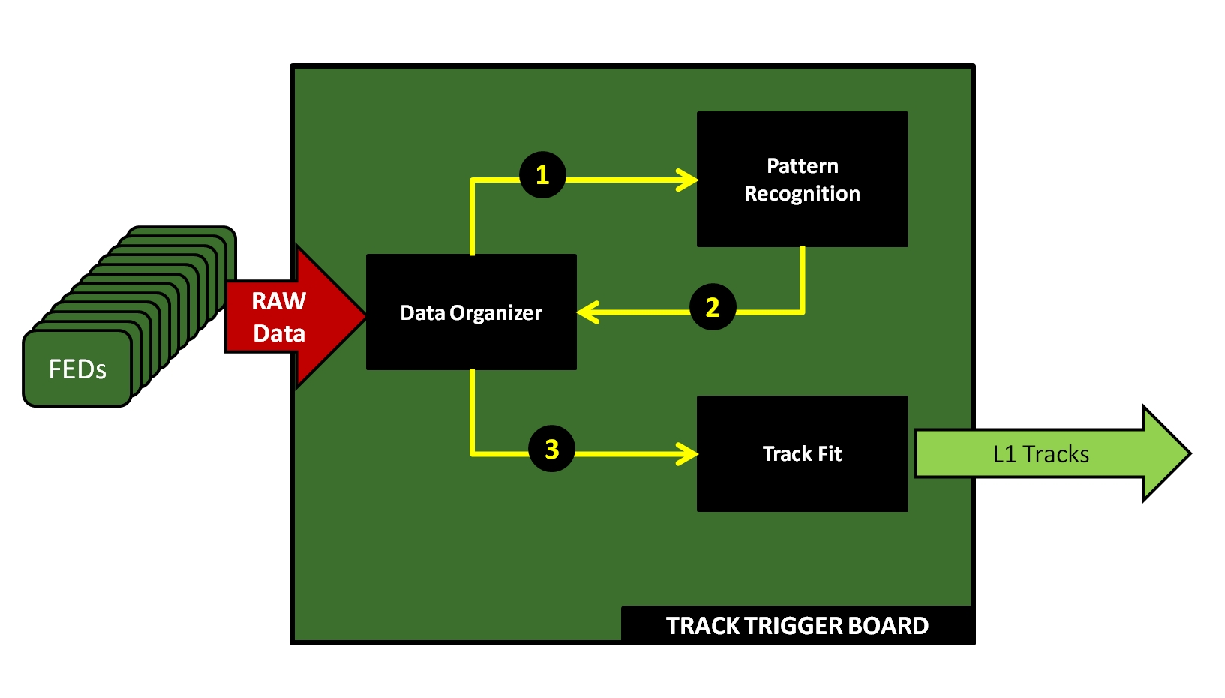
\includegraphics[width=0.5\columnwidth]{Plots/L1TTrigPrinciple.eps}
\caption{Hardware tracking principle}
\label{fig:L1TT_principle}
\end{figure}

\noindent Hardware-based tracking triggers were already developped in HEP experiments, in particular in the CDF experiment at Fermilab. Based on this system, the ATLAS experiment is planning to use a tracking trigger at the HLT after LHC long shutdown 2 in 2016. The working principle of these systems is sketched on Fig.~\ref{fig:L1TT_principle}. Tracker data is extracted by the FEDs and transmitted to the trigger board. Then, the data is handled by a data organization unit (DO), which extract the info necessary to the pattern recognition (PR), send it to the PR unit, and retrieve the matched patterns. The DO then sent the interesting hits to the track fit unit (TF), when the track parameters are estimated and sent to the L1 central trigger board.

\noindent In order to go at L1, one thus need the three following points: 

\begin{itemize}
\item A fast front-end readout system able to extract quickly all the data contained in the tracking detectors.
\item A system performing a fast pattern recognition.
\item A system performing a fast track fit.
\end{itemize}

\subsection{Interfaces}

\subsection{System architecture}

The associative memory system performs pattern recognition by comparing hits (stubs) with a reduced resolution with a large number
of prestored patterns almost in real time. 

The system is composed of mainly three parts: a data formatter (DF), which prepares the data at the reduced granularity to be transferred 
to the Associative Memory chip (AMchip), where the comparison with the patterns is performed and a list of matched patterns
is returned back. The hits at full granularity are then retrieved from the DF for the final track fitting stage (TF).

The reduced granularity compromises between the need to reduce to a manageable number of patterns to be stored in the AMchips, 
and the task of reducing the number of combinatorics in the Track Fitter stage. The AMchip stage thus overcomes the difficulties
of an approach based entirely on a fast processors architecture.

We will discuss the different tasks and their impact on the latency of the overall system. We will further address
a possible "state of the art" approach and what are the relevant directions of R\&D towards the final approach.


\subsubsection{The Data organizer}

\subsubsection{The AM chip}

The AMchip is based on an array of CAM cells. Columns of vertical buses distribute (bitlines) the hit information from each 
tracker layer to rows which contain the patterns. The rows perform writing of the patterns in the cell memory and matching 
functions. In the current AM06chip design, each bitline bus is composed of 18 bits in a hit and 18 corresponding inverted bits.
Every row is organized in sub-blocks of 8 CAMs cells (layer block), which is suited for the needs of FTK. Eventually these
will become equal to the number of needed layers of the CMS tracker. A pattern is a collection of 8 layer blocks, thus allowing
the identification of tracks crossing up to 8 layers. A logic is implemented to allow pattern matching with a pre-defined 
number of minimum blocks (8 or at least 7, for instance). The hit positions are received over 8 input buses of 15 bits each,
thus allowing a maximum of approximately 32K positions per each layer. The choice of 15 bits is taylored to the needs of FTK,
and could possibly be optimized for CMS. Actually of the 18 CAM cells each storing one bit, FTK uses 12 to store the 
12 most significant bits of the word, and 6 are used in 3 pairs and used a ternary cells, allowing for 0, 1 or X values, the 
X value meaning "don't care", so that the hits present on the hit bus will match the stored word regardless of the values
of the bits set to X. 


\subsection{Technical demonstrator concept}


\clearpage
